\subsection{Semantic Feature}
For semantic features, we've explored features related to content/stop words and the features about word pairs.\\\\
%\begin{enumerate}
%  \item Features about content/stop words.\\
%\\Stop words are word which are filtered out before or after processing of natural language data. We use a stop words list 98 common stop words.\\
%\\Content words are words such as nouns, most verbs, adjectives, and adverbs that refer to some object, action, or characteristic. We generate a content word list using the training data according to words? frequency. We retrieved the words ranks top (using a threshold) and removed stop words.\\
%    \item Feature about word pairs
%\end{enumerate}
\textbf{1. Features about content/stop words} 
\\\\Stop words are word which are filtered out before or after processing of natural language data. We use a stop words list 98 common stop words.\\
\\Content words are words such as nouns, most verbs, adjectives, and adverbs that refer to some object, action, or characteristic. We generate a content word list using the training data according to words? frequency. We retrieved the words ranks top (using a threshold) and removed stop words.\\\\
\textbf{2. Feature about word pairs}
\\\\We use Yule's measure of association as measuring the correlation between word pairs.[1] The measure of semantic association will be defined based on the contingency table below.
\begin{figure*}
\centering  
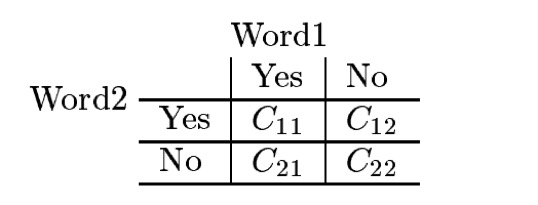
\includegraphics[width = 0.4\linewidth]{./FIG/030/contigency}\hfill
\label{fig:020feature}
\end{figure*}
For each word pair, $C_{11}$ is the count of sentences in the training corpus that contains the word pair; $C_{12}$ is the 
subtraction of the count of sentences contains word1 and $C_{11}$; $C_{21}$ is the subtraction of the count of sentences contains word2 and $C_{11}$; $C_{22}$ is the total number of sentences subtracting $C_{11}$, $C_{12}$ and $C_{21}$.\\
\\Then we calculate the Q-statistics as the correlation value between word pairs:
\begin{equation}
	Q=\frac{C_{11}C_{22} - C_{12}C_{21}}{C_{11}C_{22} + C_{12}C_{21}}
\end{equation}
The higher value of Q, the stronger the correlation between the two words.\\\\
Based on the above two categories, we designed our features as:\\\\



\subsection{Syntactic Feature}


\subsection{Statistical Feature}